\section{Perturbation at branching time}
\label{app:perturb_branching_time}
As mentioned in sections~\ref{sec:ams} and~\ref{sec:cloning}, the application of the \ac{ams} and the cloning algorithm to deterministic systems require the the addition of a perturbation to the initial condition of
resampled trajectories.
In the absence of any perturbation, the resampling would not yield new trajectories, but instead exact copies of the trajectories the resampling is based on.

The state of the flow at any point in time is given by the velocity field and the pressure $(\mathbf{u}, p)$, where the dependence on time of both variables is implicit.
A general strategy for perturbing the state of the flow is to construct a perturbative divergence free field $\delta \mathbf{u}$ and corresponding $\delta p$ solution of the
Poisson equation.
In the context of the \ac{lbm} however, the state of the system is described at a mesoscopic level by the ensemble the populations $\{f_k(x_j, y_j)\}_{0\le k \le 8, 0 \le i <N_x, 0 \le j < N_y}$.
A consequence is that, from the knowledge of a macroscopic state ($(\mathbf{u}+\delta \mathbf{u}, p + \delta p)$, it is difficult to obtain the mesoscopic state from with the \ac{lbm} model can be initialised.

In this work we work around this issue by designing the perturbative directly at the level of the mesoscopic populations.
At each lattice site $\mathbf{x}$, the populations ${f_i}_{0\le i \le 8}$ are replaced by
\begin{equation}
  f_{i}(\mathbf{x}) \longrightarrow f_i(\mathbf{x}) + \epsilon \sum_{n=1}^{N} \alpha_{n}f_{i}^{n}(\mathbf{x}), \,\,\, 1\leq i \leq 9,
  \label{eq:perturb_pop}
\end{equation}
with the set $\{\alpha_n\}_{1\leq m \leq N}$ drawn uniformly from $[0,1]$ and $\epsilon$ the amplitude of the perturbation. The perturbed populations are then rescaled so that no mass is added in the system.
For more details concerning this procedure, see appendix C of~\cite{lestang:tel-01974316}
In other words obtained as a linear combination of $N$ solutions $\{f_i^{(n)}\}_{1\le n \le N}(\mathbf{x})$ of the numerical model~\eqref{eq:lbe}.
Note that, the Lattice Boltzmann Equation~\eqref{eq:lbe} is not linear, and therefore a linear combination of solutions can be assimilated as a solution of the numerical model.
However, nonlinearities in~\eqref{eq:lbe} are located in the equilibrium distributions~\eqref{eq:lbe_eq}, and are of order of the Mach number $\mathbf{u}/c_s$ that is kept small compared to $1$, see section~\ref{sec:test_flow}.

\begin{figure}
  \centering
  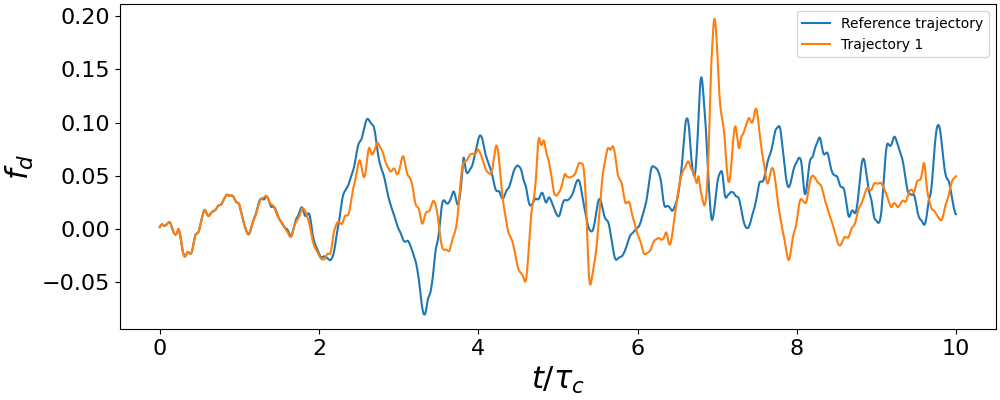
\includegraphics[width=.7\linewidth]{effect_of_perturbation/effect_of_perturbation}
  \caption[Illustration of the perturbation of the initial condition]{The blue line shows the evolution of the drag acting on the obstacle over time for a simulation initialised on a given initial condition. The second line represents the evolution of the drag for a simulation initialised on the same initial condition, however slightly perturbed as described in this appendix. $N=10$, $\epsilon=0.002$}
  \label{fig:effect_of_perturbation}
\end{figure}

In this work, we chose $N = 10$ and $\epsilon = 0.002$.
Figure~\ref{fig:effect_of_perturbation} illustrate the effect of applying a small perturbation on the evolution of the drag acting on the square obstacle.
The value of $\epsilon$ was chosen so that the perturbation does not impact the statistics of the drag.
In order to check this assumption, we generated a timeseries of duration $T_{tot} = 10^5 \tau_c$, and introduced a perturbation with $\epsilon = 0.002$ with a period $\tau = \tau_c / 2$, mimicking the perturbation of clones in the cloning algorithm.
Figure~\ref{fig:pdf_drag_with_perturbation} shows that the correct statistics are obtained even in presence of this slight perturbation.

\begin{figure}
  \centering
  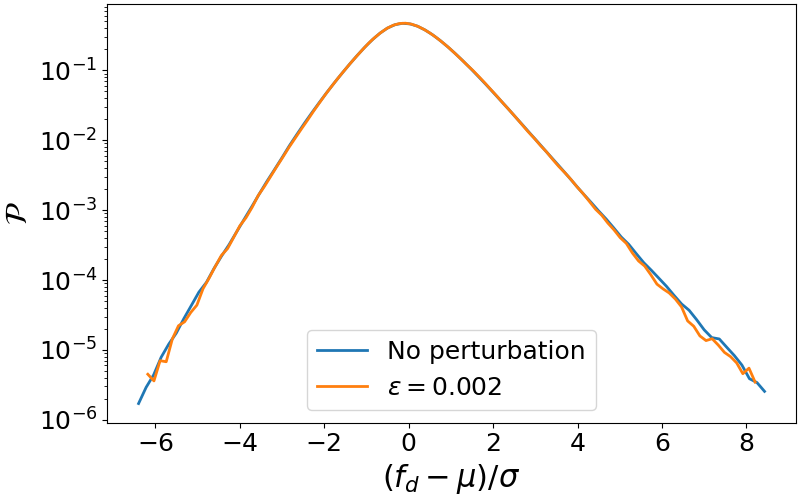
\includegraphics[width=.7\linewidth]{pdf_drag_with_perturbation/pdf_drag_with_perturbation}
  \caption{Estimation of the \ac{pdf} with and without periodic perturbations}
  \label{fig:pdf_drag_with_perturbation}
\end{figure}

%%% Local Variables:
%%% mode: latex
%%% TeX-master: "draft_p2_jfm"
%%% End: